
%(BEGIN_QUESTION)
% Copyright 2014, Tony R. Kuphaldt, released under the Creative Commons Attribution License (v 1.0)
% This means you may do almost anything with this work of mine, so long as you give me proper credit

Beregn total impedans fra disse to induktorene ved sinusformet signal med frekvens 60 Hz:

$$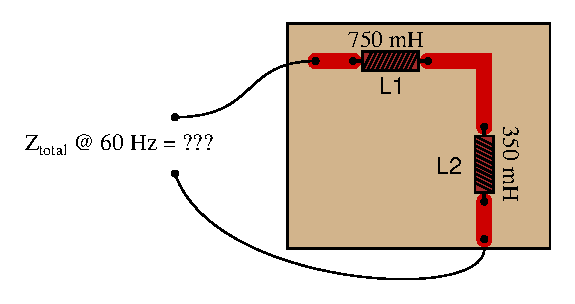
\includegraphics[width=15.5cm]{i01031x01.eps}$$

Vis arbeidet med to ulike strategier:

\begin{itemize}
\item{} Beregn total induktans ($L_{total}$) først, deretter total impedans ($Z_{total}$).
\item{} Beregn individuelle impedanser først ($Z_{L1}$ og $Z_{L2}$), deretter total impedans ($Z_{total}$).
\end{itemize}

Gir disse strategiene samme verdi? Hvorfor/hvorfor ikke?

\underbar{file i01031}
%(END_QUESTION)





%(BEGIN_ANSWER)

\noindent
{\bf Første strategi:}

$L_{total} = 1.1 \hbox{ H}$

$X_{total} = 414.7 \> \Omega$

${\bf Z_{total}} = 414.7 \> \Omega \> \angle \> 90^o$ eller ${\bf Z_{total}} = 0 + j414.7 \> \Omega$

\vskip 10pt

\goodbreak

\noindent
{\bf Andre strategi:}

$X_{L1} = 282.7 \> \Omega$ \hskip 10pt ${\bf Z_{L1}} = 282.7 \> \Omega \> \angle \> 90^o$

$X_{L2} = 131.9 \> \Omega$ \hskip 10pt ${\bf Z_{L2}} = 131.9 \> \Omega \> \angle \> 90^o$

${\bf Z_{total}} = 414.7 \> \Omega \> \angle \> 90^o$ eller ${\bf Z_{total}} = 0 + j414.7 \> \Omega$

%(END_ANSWER)





%(BEGIN_NOTES)

Hensikten er å vise at flere fremgangsmåter kan gi samme korrekte totalimpedans, og dermed gi en god måte å kontrollere eget arbeid på.

%INDEX% Electronics review: AC reactance and impedance

%(END_NOTES)

